\title{Entrevista}
\subtitle{com Paulo Ivonir Gubiani}
\maketitle
\begin{wrapfigure}{l}{0.15\textwidth}
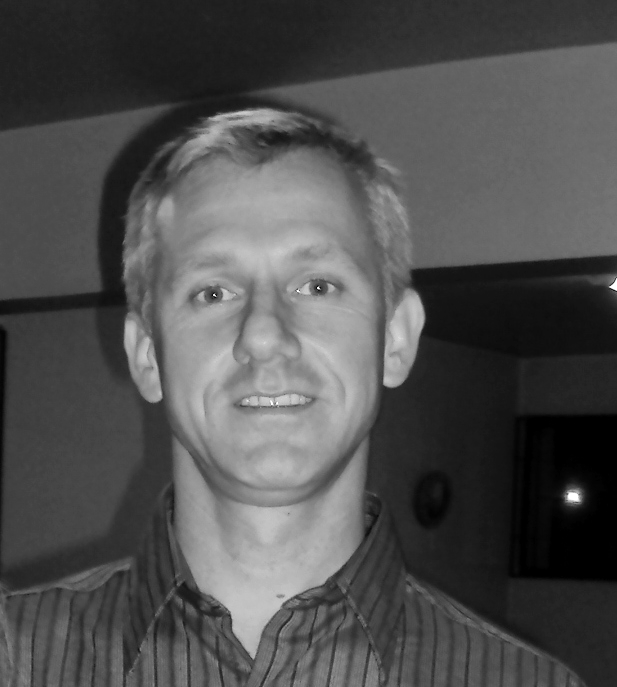
\includegraphics[width=0.15\textwidth]{figuras/foto-paulo}
\end{wrapfigure}

Nesta edição da \pedometria, entrevistamos o Professor Doutor Paulo Ivonir Gubiani para falar um pouco sobre sua experiência em modelagem matemática na área de Física do Solo, sua opinião com relação as pesquisas na área de modelagem, dificuldades e perspectivas futuras no Brasil. O Dr. Paulo atualmente é docente no Departamento de Solos - Setor de Física do Solo da Universidade Federal de Santa Maria (UFSM). Sua formação pós ensino médio foi realizada na UFSM, onde cursou Agronomia. Na mesma universidade fez seu mestrado e doutorado em Ciência do Solo na área de Processos Físicos e Morfogenéticos do Solo.

\pergunta{O que levou você a se interessar e estudar temas relacionados à modelagem matemática de dados ambientais, em especial, processos relacionados ao solo?}

\resposta{Paulo}{Penso que o estudo sobre modelagem matemática na área que atuo, isto é, Física do Solo, não é uma questão apenas de gosto ou interesse, mas sim de necessidade. O solo é um sistema aberto e dinâmico, e medidas pontuais de suas propriedades informam apenas estados do sistema. Na ciência, a medição constitui uma etapa fundamental, que é a observação. Porém, o ``fazer'' ciência vai muito além da observação. Em sistemas abertos e dinâmicos o principal interesse e função do pesquisador é conhecer a evolução do sistema no tempo, suas causas e consequências. As medições conseguem descrever o estado do sistema num instante de tempo, mas não permitem prever estados e consequências futuras. Com a modelagem matemática, estados do sistema podem ser simulados a partir do conhecimento da inter-relação de suas variáveis. A modelagem não visa substituir a medição, mas sim fornecer um valor aproximado para variáveis que, por razões técnicas ou físicas, não podem ser medidas (por exemplo, estado de um sistema no futuro). No que se refere ao solo, previsões aproximadas de erosão do solo, estoque de carbono, transferência de compostos abióticos e bióticos entre ambientes, armazenamento de água no solo, emissão de gases de efeito estufa, entre outros, são de grande utilidade para que cientistas do solo projetem as consequências para a humanidade do atual modo de utilização do solo. A modelagem é, certamente, uma simplificação de um sistema real. Contudo, ela é uma simplificação integradora. Quando modelamos, conectamos os componentes de um sistema e analisamos o sistema como um todo a partir das relações naturalmente indissociáveis de seus componentes. Quando não modelamos, simplificamos ainda mais o sistema, limitamos e tornamos mais falíveis as previsões sobre o comportamento do sistema.}

\pergunta{Quais os projetos de pesquisa que você está desenvolvendo ou participando relacionados à modelagem e estimação de propriedades do solo ou processos que ocorrem no solo?}

\resposta{Paulo}{No momento, estou participando diretamente de um estudo de dissertação sobre modelagem da infiltração de água no solo. Nosso objetivo é desenvolver uma aplicação numérica do modelo de Green-Ampt para perfil de solo multicamada, sem limitação do número de camadas de solo com distintas propriedades hidráulicas e sob condições de chuva natural. O estudo está na fase de obtenção de dados. As primeiras simulações com o algoritmo que criamos são promissoras, mas precisamos de mais medições para avaliação e calibração do modelo. Também auxilio uma doutoranda do Programa de Pós-Graduação em Engenharia Agrícola da UFSM, na implementação de modelos de balanço hídrico do solo, no modelo de simulação de produção da cultura da mandioca que ela está desenvolvendo.}

\pergunta{Qual sua opinião a respeito do cenário atual das pesquisas em modelagem na ciência do solo no Brasil?}

\resposta{Paulo}{Minha opinião sobre essa questão é baseada em duas análises. A primeira foi feita pelo professor Quirijn de Jong Van Lier, do CENA/USP, e foi apresentada em sua palestra no XXXIII Congresso Brasileiro de Ciência do Solo, na cidade de Uberlândia-MG, em 2011. O professor Quirijn analisou a frequência de ocorrência dos termos ``modelo'' ou ``modelagem'' nos títulos das publicações da área de física do solo em três fontes: nos resumos do XXXII Congresso Brasileiro de Ciência do Solo de 2009 (XXXII CBCS); na Revista Brasileira de Ciência do Solo (RBCS), no período de 2003 a 20011; e na Soil Science Societe American Journal (SSSAJ), no período de 2006 a 2011. Sua constatação foi que os termos ``modelo'' ou ``modelagem'' raramente apareciam nos títulos das publicações do XXXII CBCS, apareciam em menos que 5 por cento dos títulos da RBCS e em torno de 10 por centodos títulos da SSSAJ. Além disso, a comparação entre RBCS e SSSAJ demonstrou que nos dedicamos pouco ao estudo de processos e instrumentação, assuntos que antecedem e dão suporte para a modelagem. A segunda análise foi um levantamento que eu fiz também da frequência de ocorrência dos termos ``modelo'' ou ``modelagem'' nos títulos dos 221 resumos apresentados no XXXIV Congresso Brasileiro de Ciência do Solo de 2013, na comissão de física do solo. Apenas em três dos 221 títulos constava o termo ``modelagem'' (\url{http://gubianisolos.blogspot.com.br/2013/08/fisica-do-solo-apresentada-no-xxxivcbcs.html}). Esse panorama da modelagem para a Ciência do Solo no Brasil poderia ser refinado por pesquisador, usando os títulos de seus artigos cadastrados na plataforma Lattes. Caso isso fosse feito, verificaríamos que existem alguns pesquisadores que atuam com maior ênfase na modelagem em relação a outros muitos que ainda não iniciaram ou estão iniciando estudos com esse propósito.}
\vspace{5mm}
\begin{figure}[h!]
 \centering
 \includegraphics[width=0.8\textwidth]{figuras/foto-paulo-mensuration}
 \caption{Monitoramento da umidade do solo pela técnica da Reflectometria no Domínio do Tempo (TDR). Tal técnica é comumente utilizada em estudos de modelagem matemática na área de Física do Solo. Fonte: Paulo Gubiani.}
\end{figure}

\pergunta{Qual a sua opinião a respeito de assuntos como a modelagem matemática de processos e atributos do solo, geoestatística e linguagem de programação como disciplinas nos cursos de Pós-Graduação da área de solos no Brasil?}

\resposta{Paulo}{Penso que a inclusão desses conteúdos como disciplinas nos cursos de Pós-Graduação (PG) da área de solos está diretamente relacionada com o resultado técnico-científico que cada PG vislumbra e com a independência dessa produção de PG externos. Para um PG cujos professores orientadores praticam a modelagem matemática, essas disciplinas, ou algumas delas, já são ofertadas aos estudantes, porque esses conteúdos são indispensáveis para o desenvolvimento da modelagem matemática. Para um PG cujos professores orientadores não praticam a modelagem matemática, e que têm interesse em atuar nessa área, essas disciplinas teriam que ser cursadas também pelos professores. É pouco provável que alguém queira orientar uma pesquisa sobre modelagem matemática se não domina o assunto. Outro agravante é a combinação do precário embasamento matemático de estudantes de graduação que ingressam na pós-graduação em ciência do solo e o curto período de tempo que esses estudantes têm no mestrado e no doutorado para que disciplinas oferecidas na pós-graduação supram as carências e adicionem os requisitos matemáticos mínimos para a modelagem. Embora existam exceções, na maioria dos casos o que se consegue nessa condição de carência de formação é habilitar operadores de softwares de modelagem. Isso é útil para formar e/ou exportar operadores de softwares executores de simulações. Mas, se os PGs vislumbram gerar e exportar modelos, então acredito que, além de ofertar disciplinas na pós-graduação, é essencial o fortalecimento da formação matemática, estatística e de programação na graduação e, sobretudo, nos grupos de pesquisa durante a iniciação científica.}

\pergunta{Pela sua experiência na área de modelagem ambiental, quais as principais dificuldades e desafios encontrados para os pesquisadores brasileiros desenvolverem seus trabalhos nessa área?}

\resposta{Paulo}{Minha experiência é bem pequena se comparada à experiência de pesquisadores que trabalham com modelagem há bastante tempo. Porém, o que tenho sentido e notado até o momento coincide com a opinião de pesquisadores experientes no assunto. Sabe-se que o pesquisador ou seu grupo deve estar munido das habilidades necessárias para a modelagem. Nesse ponto, ele deve compreender bem conceitualmente o sistema físico que quer modelar, conhecer ou desenvolver possibilidades matemáticas para descrição das relações dos componentes do sistema e conectar toda a estrutura matemática numa unidade que permite a reprodução aproximada do sistema. Além disso, os pesquisadores devem efetuar a calibração e validação dos seus modelos, o que exige medições no sistema que está sendo modelado. Os desafios principais dependem do sistema que está sendo modelado. Pode ser a formação matemática e de programação (quando se quer criar ou modificar um modelo existe) a formação de equipes multidisciplinares (modelagem de sistemas multicompartimentais) ou a formação de grupo de pesquisa e aquisição de equipamentos (monitoramento para medições de sistemas multicompartimentais e espacialmente abrangentes). Do ponto de vista da capacitação, a maioria dos estudantes nas universidades tem um computador pessoal, ferramenta que facilita o aprendizado de modelagem matemática. Porém, a popularização do computador é recente no Brasil. Além disso, os estudantes dos cursos de graduação que mais candidatos oferecem para a pós-graduação em ciência do solo, embora tenham a ferramenta computacional, dispõem de pouco ou nada de disciplinas sobre modelagem matemática e programação. Outro grande desafio é externo ao escopo da modelagem. Trata-se da motivação da produção de dissertações, teses e artigos científicos num modelo que prevalece o critério da quantidade. Logicamente se produz em maior quantidade quanto mais simples de serem executadas forem as pesquisas. A modelagem se ocupa em explicar sistemas, o que requer a descrição de processos, trabalho que é bem mais complexo do que medir e discutir relações entre propriedades num período pequeno de tempo. Fazendo uma analogia à expressão ``publique ou pereça'', usada para indicar a atual situação da ciência, basta fazer uma consulta nos currículos Lattes dos pesquisadores que se perceberá claramente que os pesquisadores ``perecem'' com a modelagem e ``publicam'' com a relação estatística de propriedades.}

\pergunta{Qual a sua opinião a respeito da interdisciplinaridade nos grupos de pesquisa da área de solos para desenvolver trabalhos que contribuam para meio científico? Em sua opinião, existe interdisciplinaridade nos grupos de pesquisa do Brasil? Sim ou Não? Por quê?}

\resposta{Paulo}{O conceito de interdisciplinaridade ainda segue em construção e está sujeito a interpretações distintas, como mobilização dos conteúdos de duas ou mais disciplinas, fusão de conteúdos de disciplinas em uma nova, etc. O primeiro caso é o que mais acontece nos grupos de pesquisa, com intensidade e abrangência variável. A solução de problemas simples depende menos da mobilização de conhecimentos de várias disciplinas, ao passo que problemas complexos se inserem num escopo interdisciplinar. Porém, qualquer conhecimento novo é uma contribuição importante da ciência para ampliar o corpo de conhecimentos existente e não somente os que resultam de interação interdisciplinar. A prática da interdisciplinaridade vai avançando na medida em que os grupos se consolidam, os projetos de pesquisa passam a tratar de problemas mais abrangentes, necessitam e reúnem conhecimentos de várias áreas, recebem mais suporte financeiro e estrutural e consolidam parcerias nacionais e internacionais. Nos últimos anos, interações e cooperações aumentaram, tanto em nível nacional como internacional (verificar a seção acesso à informação no site da CAPES) o que cria espaço para a mobilização de conteúdos de várias disciplinas para a solução de problemas. Há vários exemplos no Brasil da prática interdisciplinar resultante dessas interações, como a formação de grupos de estudo dos sistemas integrados lavoura-pecuária ou lavoura-pecuária-floresta, grupos de estudo de processos hidrossedimentológicos em escala de bacia hidrográfica e grupos dedicados ao mapeamento digital de solo. Nesses estudos, o que guia o pesquisador é a noção holística e sistêmica, de integração dos componentes de um sistema, do estudo do todo a partir de suas partes. Ainda há muito trabalho acadêmico para ser feito para que essas e muitas outras áreas de conhecimento sejam cobertas com pesquisas integradoras. Para esse propósito, incentivar estudantes a aprenderam modelagem matemática é uma ótima iniciativa para exercitar essa noção integradora e interdisciplinar.}
%%% Local Variables:
%%% mode: latex
%%% TeX-master: 4rd-edition.tex
%%% End: